%
%  exercise-1.tex
%  artificial intelligence
%
%  Created by Illya Starikov on 01/17/18.
%  Copyright 2018. Illya Starikov. All rights reserved.
%

\RequirePackage[l2tabu, orthodox]{nag} \documentclass[12pt]{scrartcl}

\newcommand{\exercisenumber}{6}
\newcommand{\duedate}{July 27\textsuperscript{th}, 2018}
\usepackage{amssymb,amsmath,verbatim,graphicx,microtype,upquote,units,booktabs,akkwidepage}

\newcommand{\chapterNumber}[1]{
    \setcounter{section}{#1}
    \addtocounter{section}{-1}
}
\usepackage[shortlabels]{enumerate}
\usepackage{multicol}

\definecolor{dkgreen}{rgb}{0,0.6,0}
\definecolor{gray}{rgb}{0.5,0.5,0.5}
\definecolor{mauve}{rgb}{0.58,0,0.82}

\lstdefinelanguage{Julia}%
  {morekeywords={abstract,break,case,catch,const,continue,do,else,elseif,%
      end,export,false,for,function,immutable,import,importall,if,in,%
      macro,module,otherwise,quote,return,switch,true,try,type,typealias,%
      using,while},%
   sensitive=true,%
   alsoother={$},%
   morecomment=[l]\#,%
   morecomment=[n]{\#=}{=\#},%
   morestring=[s]{"}{"},%
   morestring=[m]{'}{'},%
}[keywords,comments,strings]%

\lstdefinestyle{r}{
  language=R,                     % the language of the code
  basicstyle=\ttfamily\footnotesize,       % the size of the fonts that are used for the code
  numbers=left,                   % where to put the line-numbers
  numberstyle=\tiny\color{gray},  % the style that is used for the line-numbers
  stepnumber=1,                   % the step between two line-numbers. If it's 1, each line
                                  % will be numbered
  numbersep=5pt,                  % how far the line-numbers are from the code
  backgroundcolor=\color{white},  % choose the background color. You must add \usepackage{color}
  showspaces=false,               % show spaces adding particular underscores
  showstringspaces=false,         % underline spaces within strings
  showtabs=false,                 % show tabs within strings adding particular underscores
  frame=single,                   % adds a frame around the code
  rulecolor=\color{black},        % if not set, the frame-color may be changed on line-breaks within not-black text (e.g. commens (green here))
  tabsize=2,                      % sets default tabsize to 2 spaces
  breaklines=true,                % sets automatic line breaking
  breakatwhitespace=false,        % sets if automatic breaks should only happen at whitespace
  keywordstyle=\color{blue},      % keyword style
  commentstyle=\color{dkgreen},   % comment style
  stringstyle=\color{mauve}      % string literal style
}

\lstdefinestyle{julia}{
  language=Julia,                     % the language of the code
  basicstyle=\ttfamily\footnotesize,       % the size of the fonts that are used for the code
  numbers=left,                   % where to put the line-numbers
  numberstyle=\tiny\color{gray},  % the style that is used for the line-numbers
  stepnumber=1,                   % the step between two line-numbers. If it's 1, each line
                                  % will be numbered
  numbersep=5pt,                  % how far the line-numbers are from the code
  backgroundcolor=\color{white},  % choose the background color. You must add \usepackage{color}
  showspaces=false,               % show spaces adding particular underscores
  showstringspaces=false,         % underline spaces within strings
  showtabs=false,                 % show tabs within strings adding particular underscores
  frame=single,                   % adds a frame around the code
  rulecolor=\color{black},        % if not set, the frame-color may be changed on line-breaks within not-black text (e.g. commens (green here))
  tabsize=2,                      % sets default tabsize to 2 spaces
  breaklines=true,                % sets automatic line breaking
  breakatwhitespace=false,        % sets if automatic breaks should only happen at whitespace
  keywordstyle=\color{blue},      % keyword style
  commentstyle=\color{dkgreen},   % comment style
  stringstyle=\color{mauve}      % string literal style
}

\begin{document}
\maketitle

\section{Support Vectors}
\lstinputlisting[style=r]{src/problem-1.r}

The output is as follows:

\begin{verbatim}
 Setting default kernel parameters
[[1]]
  X1 X2
2  2  1
3  4  2

[1] 1
[1] -1
\end{verbatim}

\section{Bayes Network}
\lstinputlisting[style=r]{src/problem-2.r}

The network looks as follows:

\begin{figure}[H]
    \centering
    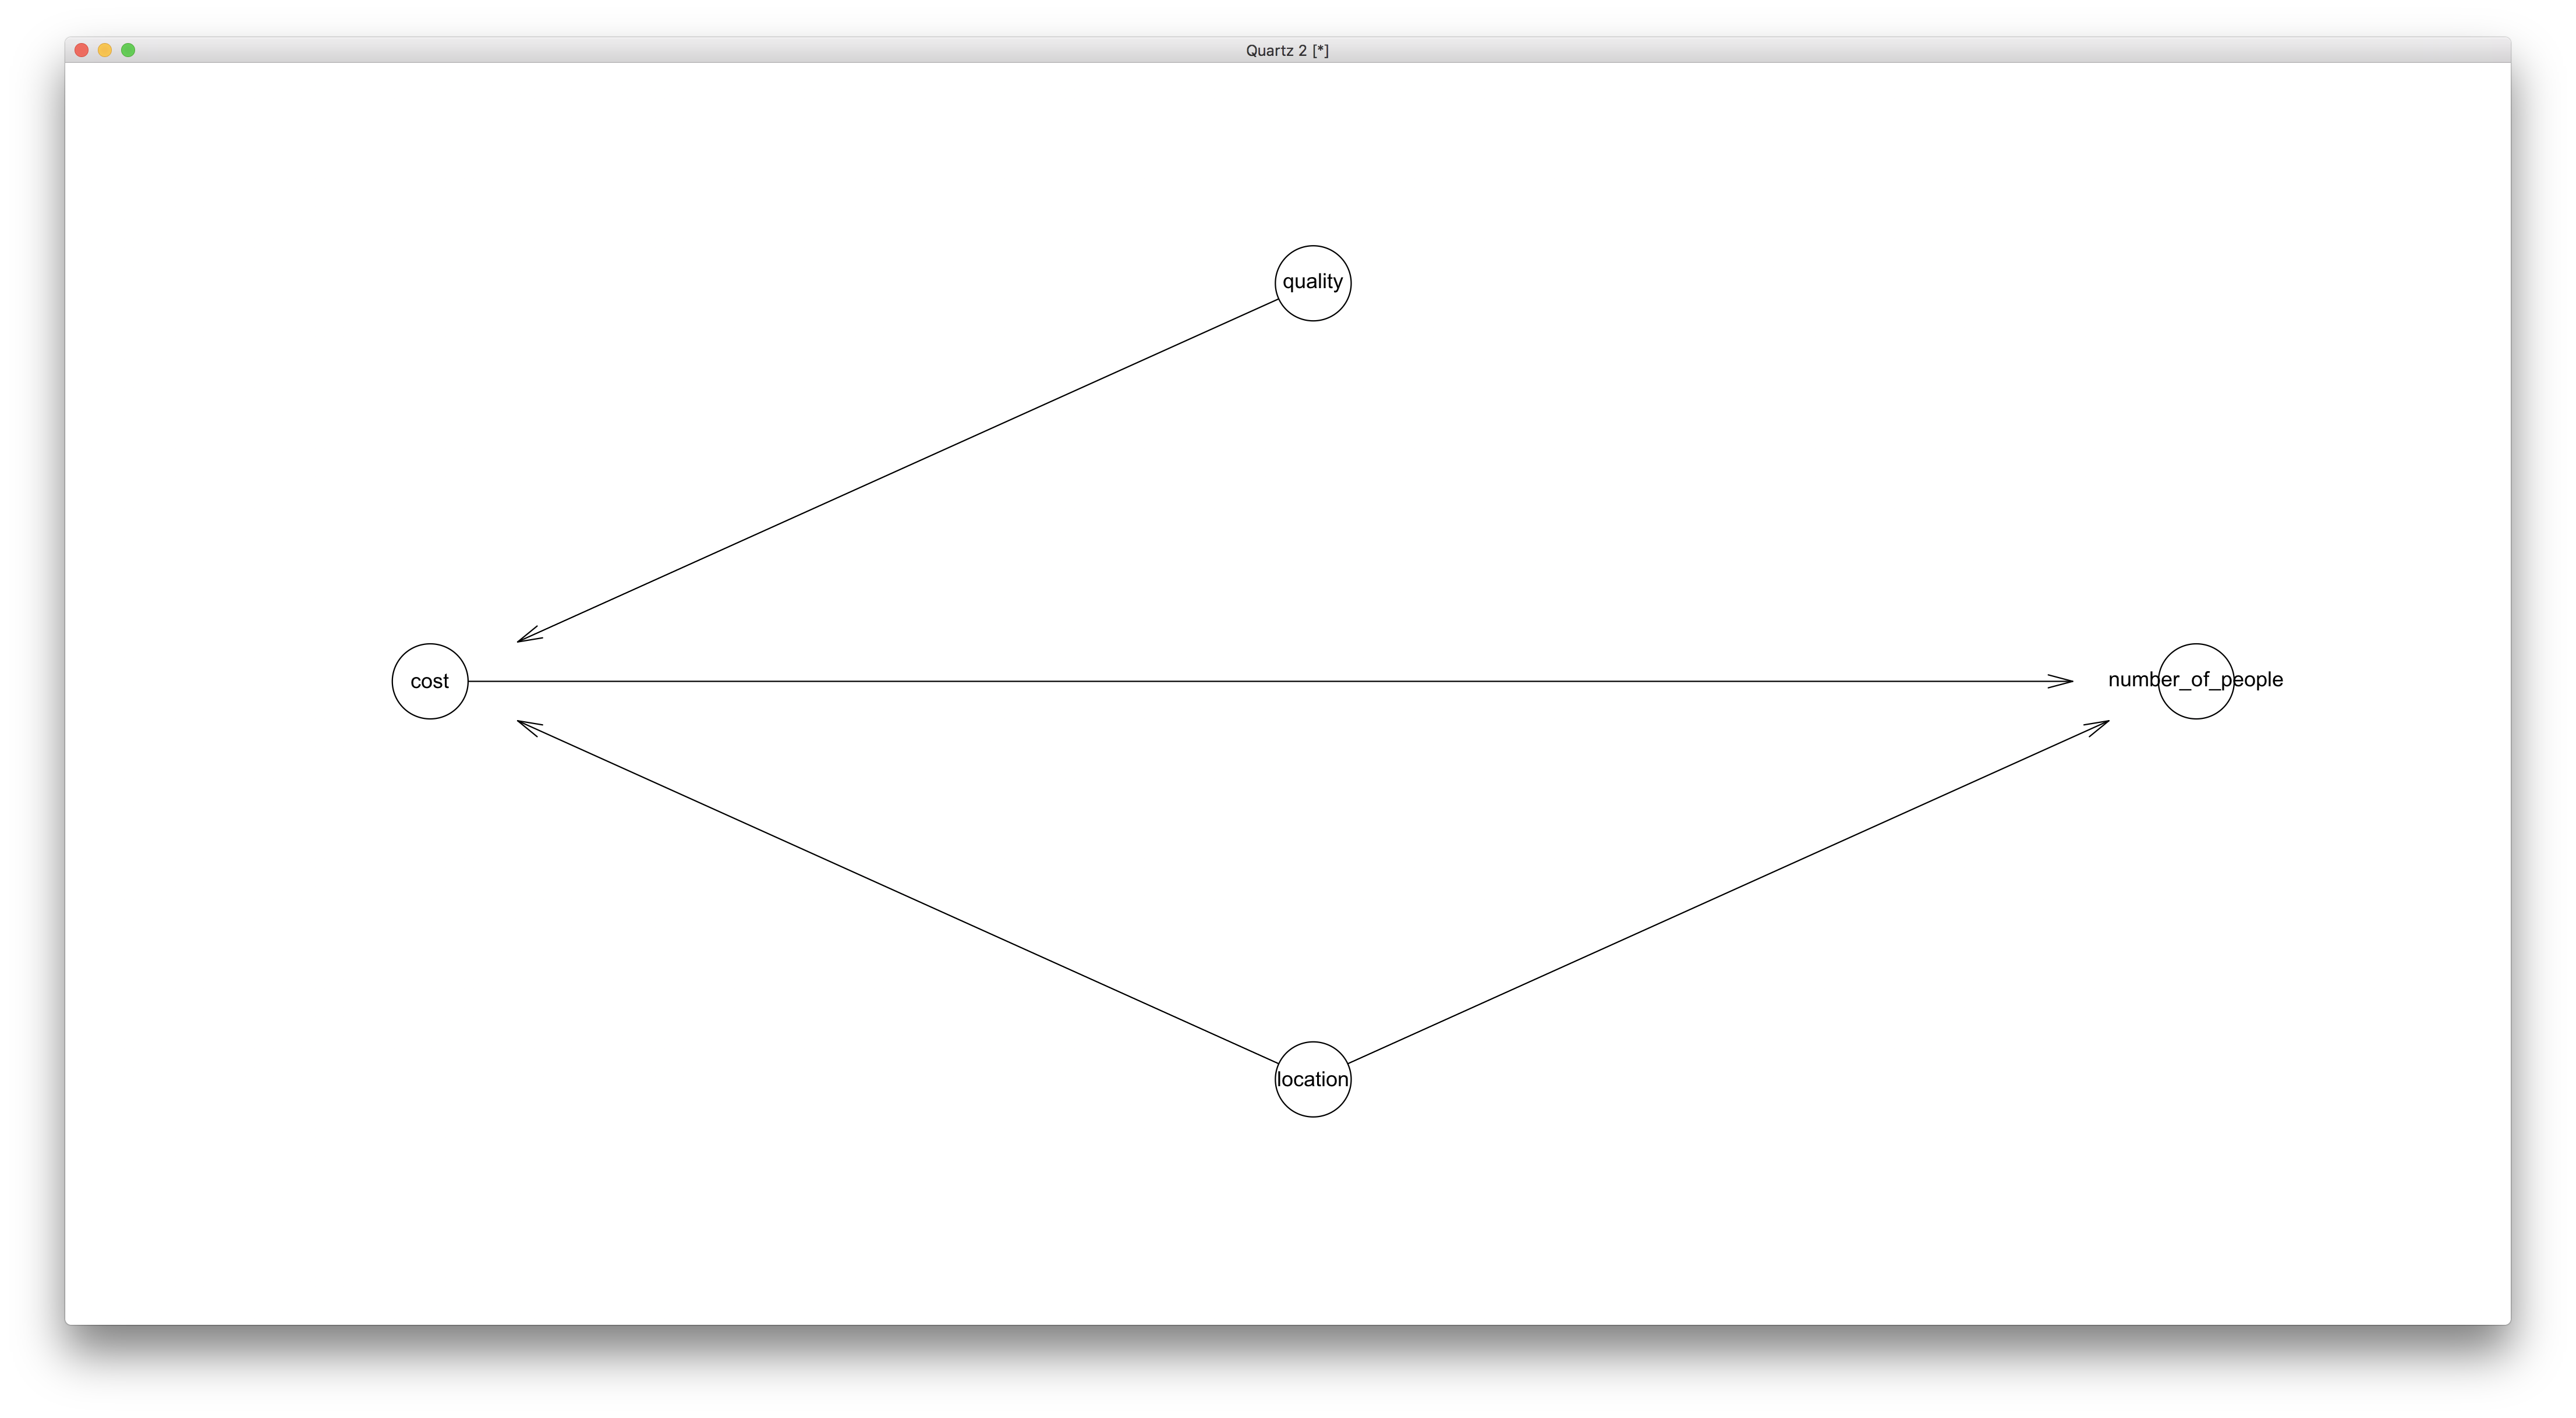
\includegraphics[width=0.8\linewidth]{assets/dag}
\end{figure}

The output looks as follows:

\begin{verbatim}
$location
location
Good  Bad
 0.6  0.4

$quality
quality
  Good Normal    Bad
   0.3    0.5    0.2

$cost
, , location = Good

      quality
cost   Good Normal Bad
  High  0.8    0.6 0.1
  Low   0.2    0.4 0.9

, , location = Bad

      quality
cost   Good Normal  Bad
  High  0.6    0.6 0.05
  Low   0.4    0.4 0.95


$number_of_people
, , location = Good

                cost
number_of_people High Low
            High  0.6 0.8
            Low   0.4 0.2

, , location = Bad

                cost
number_of_people High Low
            High  0.1 0.6
            Low   0.9 0.4



prediction Good Normal
    Good      0      0
    Normal    1      1
    Bad       0      0
[1] Normal Normal
Levels: Good Normal Bad
\end{verbatim}

\section{DBScan}
\lstinputlisting[style=julia]{src/problem-3.jl}
\begin{verbatim}
Clustering.DbscanResult(
    [1, 5, 7, 12, 13, 14, 15, 16, 17, 22, 23, 24, 25, 29, 31],
    [1, 1, 1, 1, 2, 1, 3, 1, 1, 1, 1, 4, 5, 6, 7, 8, 9, 1, 1, 1,
        1, 10, 11, 12, 13, 1, 1, 1, 14, 1, 15, 1],
    [18, 1, 1, 1, 1, 1, 1, 1, 1, 1, 1, 1, 1, 1, 1])
\end{verbatim}

\textbf{Gadfly could not produce a graph.}

\section{Decision Tree}
\lstinputlisting[style=julia]{src/problem-4.jl}

\begin{verbatim}
Feature 3, Threshold 118.0
L-> Feature 3, Threshold 96.0
    L-> Feature 3, Threshold 65.5
        L-> Feature 1, Threshold 1.5
            L-> 33.9 : 1/1
            R-> Feature 3, Threshold 57.0
                L-> 30.4 : 1/1
                R-> 24.4 : 1/1
        R-> Feature 3, Threshold 92.0
            L-> Feature 1, Threshold 1.5
                L-> 27.3 : 1/2
                R-> 26.0 : 1/1
            R-> 22.8 : 2/2
    R-> Feature 1, Threshold 3.0
        L-> Feature 3, Threshold 107.0
            L-> Feature 2, Threshold 5.0
                L-> 21.5 : 1/1
                R-> 18.1 : 1/1
            R-> Feature 4, Threshold 4.5
                L-> 21.4 : 2/2
                R-> 30.4 : 1/1
        R-> 21.0 : 2/2
R-> Feature 3, Threshold 192.5
    L-> Feature 2, Threshold 7.0
        L-> Feature 4, Threshold 4.5
            L-> 17.8 : 1/2
            R-> 19.7 : 1/1
        R-> Feature 1, Threshold 2.5
            L-> Feature 3, Threshold 162.5
                L-> 15.2 : 1/2
                R-> 19.2 : 1/2
            R-> 16.4 : 1/3
    R-> Feature 3, Threshold 237.5
        L-> Feature 3, Threshold 222.5
            L-> 10.4 : 2/2
            R-> 14.7 : 1/1
        R-> Feature 3, Threshold 254.5
            L-> 14.3 : 1/2
            R-> Feature 3, Threshold 299.5
                L-> 15.8 : 1/1
                R-> 15.0 : 1/1
\end{verbatim}

\section{KMeans}
\lstinputlisting[style=julia]{src/problem-5.jl}
\begin{verbatim}
  Iters               objv        objv-change | affected
-------------------------------------------------------------
      0       1.000000e+02
      1       4.880000e+01      -5.120000e+01 |        0
      2       4.880000e+01       0.000000e+00 |        0
K-means converged with 2 iterations (objv = 48.80000000000001)
Assignments: [1 1 1 1 2 1 3]
Counts: [5 1 1]
\end{verbatim}

\end{document}
